\section{Biographie du Développeur}\label{chap:biographie}
\vspace{-0.9em}

\begin{center}
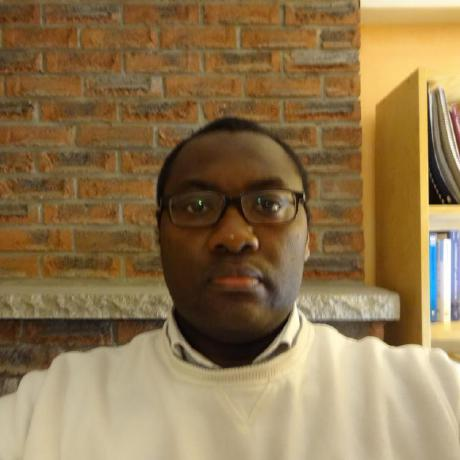
\includegraphics[scale=0.32]{../../francais/images/XavierNOUNDOU-2}
\captionof{figure}{Portrait du DR. XAVIER.\label{fig:xaviernoumbis}}
\end{center}

\textbf{\myfullacademicname} est CHRÉTIEN de confession
(église évangélique du cameroun),
Camerounais, né le $16$~Septembre $1983$ à
DOUALA (région du LITTORAL, CAMEROUN).

Le DR. Xavier est \textit{DOCTEUR/PH.D. en Génie Informatique}
(construction du logiciel, et test) depuis le $18$~Novembre~$2020$
grâce à ses résultats probants dans l'ingénierie
professionnelle du logiciel (\yerotherpblack), et dans la recherche
fondamentale et appliquée en génie informatique
(vérification statique du code \cplusplus, avec des applications
en sécurité, et en assurance qualité du logiciel):

\begin{enumerate}
%	\itemsep -0.7em
	\item "Context-Sensitive Staged Static Taint Analysis
			For C using LLVM"
		\begin{enumerate}[1.]
			\itemsep -0.7em
			\item code source en \cplusplus: \url{http://github.com/xnoumbissinoundou/yeroth-saint}
			\item texte complet (publié le $1^\text{er}$~Juillet, $2015$): \url{http://archive.org/details/saint_201507}.
		\end{enumerate}		 

	\item "YEROTH-ERP-3.0": \url{http://archive.org/details/yeroth-erp-3-0-info-english}.\\
\end{enumerate}


LE DR. XAVIER À $1$ GRADE ACADÉMIQUE ET PROFESSIONNEL
DE ''DIPLOM--INFORMATIKER~(DIPL.--INF.)''
(INGÉNIEUR DE CONCEPTION EN INFORMATIQUE) de
\textbf{l'\bremenu, BRÊME, BREMEN, ALLEMAGNE}
($25$~MAI~$2007$).

